%-------------------- Packages --------------------%

\documentclass[11pt,a4paper]{report}
\usepackage[utf8]{inputenc}
\usepackage[french]{babel}
\usepackage[T1]{fontenc}
\usepackage{amsmath} %pour les formules maths
\usepackage{amsfonts}
\usepackage{amssymb}
\usepackage{graphicx} %pour inclure des images
\usepackage{hyperref} %pour les lien URLs
\usepackage[left=2cm,right=2cm,top=3cm,bottom=3cm]{geometry}
\usepackage{pifont} %pour les puces spéciales
\usepackage{listings} %pour écrire du code
\usepackage{xcolor} %pour la mise en couleur
\usepackage{multirow} %pour les tableaux
\usepackage{bclogo} %pour des boîtes texte avec un logo


%-------------------- New Colors --------------------%

%Basic

\definecolor{purple}{rgb}{0.6, 0.2, 0.9}

%Dark
\definecolor{dkgreen}{rgb}{0,.6,0}
\definecolor{dkblue}{rgb}{0,0,.6}
\definecolor{dkyellow}{cmyk}{0,0,.8,.3}
\definecolor{dkred}{rgb}{0.6, 0, 0}


%Light
\definecolor{ltblue}{rgb}{0.67, 0.85, 0.9}
\definecolor{ltred}{rgb}{0.8, 0.32, 0.32}
\definecolor{ltgrey}{rgb}{0.94,0.94,0.94}



%-------------------- Config lstlisting --------------------%

\lstset{
language=php,
basicstyle=\ttfamily\tiny, %
identifierstyle=\color{dkred}, %
keywordstyle=\color{dkblue}, %
stringstyle=\color{dkgreen}, %
commentstyle=\it\color{gray}, %
emph=[1]{php},
emphstyle=[1]\color{black},
emph=[2]{if,and,or,else},
emphstyle=[2]\color{dkyellow},
emph=[3]{imap_open, imap_close, imap_fetch_overview, imap_check, imap_list, imap_mail_move, imap_search, imap_fetchstructure			},
emphstyle=[3]\color{dkblue},
emph=[4]{string, int, double, float, private, public, static, bool, resource, array, object},
emphstyle=[4]\color{purple},
columns=flexible, %
tabsize=2, %
extendedchars=true, %
showspaces=false, %
showstringspaces=false, %
numbers=left, %
numberstyle=\tiny, %
breaklines=true, %
breakautoindent=true, %
captionpos=b, %
backgroundcolor=\color{ltgrey}
}


\newcommand{\vf}[3]{\textcolor{dkblue}{\textit{#1}}\hspace*{.2cm}#2\vspace*{.2cm}\par\hspace*{.5cm}#3}
\newcommand{\qouv}[2]{\textcolor{dkblue}{\textit{#1}}\vspace*{.2cm}\par\hspace*{.5cm}#2}

\newcommand{\vrai}[0]{\textcolor{dkgreen}{Vrai}}
\newcommand{\faux}[0]{\textcolor{dkred}{Faux}}

\title{Préparation à l'examen d'\textit{Architecture Logicielle}}
\author{Wery Benoît}
\date{\today}

\begin{document}
\maketitle
%------------------------------------------------------------------------
\chapter{Vrai ou Faux}
%------------------------------------------------------------------------
\begin{enumerate}\setlength\itemsep{1em}
%--- 1 -------------------------------%
\item\vf{Dans une entreprise, les données vivent souvent plus longtemps que les logiciels.}
{\vrai}
{Une entreprise \textit{utilise} des logiciels et \textit{stocke} des données en veillant à garder le plus d'indépendance possible entre ces deux éléments. Ainsi, un changement d'implémentation de la structure des données ne devrait pas affecter le bon fonctionnement du logiciel.

\paragraph{}
Là où les données doivent persister dans le temps, un logiciel peut être amené à être remplacé (par obsolescance, optimisation,...)
}


%--- 2 -------------------------------%
\item\vf{Dans une entreprise, les logiciels vivent souvent plus longtemps que les données.}
{\faux}
{}


%--- 3 -------------------------------%
\item\vf{Le passage du relationnel au NoSQL se fait généralement au profit d’une diminution des garanties
relatives à la consistence des données.}
{???}
{}


%--- 4 -------------------------------%
\item\vf{Le passage du relationnel au NoSQL se fait généralement au profit d’une diminution de la
quantité de données stockables.}
{\faux}
{... stockables VS stockées...

\paragraph{}
Le NoSQL a émmergé d'un besoin de stocker de nouveaux formats de données (ex: stocker directement des objets plutôt que de devoir retrouver leur informations indépendantes pour le reconstruire), malgré la \textit{puissance} et la \textit{stabilité} des base de données relationnelles, celles-ci ne sont plus suffisantes dans certaines applications.
}


%--- 5 -------------------------------%
\item\vf{Le passage du relationnel au NoSQL se fait généralement au profit de l’abandon de la possibilité
de lire des données de manière concurrente.}
{\faux}
{Le modèle relationnel permet d'accéder de manière concurrente aux données (en R/W) via l'utilisation de \textbf{transactions}, les données sont stockées de façon consistante et persistante.

\paragraph{}
Le modèle NoSQL, quant à lui, permet un accès concurrent aux données MAIS elles ne sont pas garanties consistantes. De plus, les données d'une BDD étant stockées sur des serveurs différents (contrairement au relationnel -> 1machine/BDD), il se peut que des requêtes identiques fournissent des résultats différents. ... A VERIFIER
}


%--- 6 -------------------------------%
\item\vf{Le passage du relationnel au NoSQL se fait généralement au profit d’une diminution des garanties
relatives à la persistance des données.}
{???}
{"la gestion de la persistance des données réfère au mécanisme responsable de la sauvegarde et de la restauration des données. Ces mécanismes font en sorte qu'un programme puisse se terminer sans que ses données et son état d'exécution ne soient perdus". A VERIFIER}


%--- 7 -------------------------------%
\item\vf{Tout comme pour le relationnel, l’organisation des données en NoSQL suit un modèle mathéma-
tique rigoureux.}
{\faux}
{Là où le relationnel se base sur des modèles mathématiques standards pour définir la structure de la BDD, le NoSQL ne suit pas de schéma (ex: possibilité d'ajout de champs sans contrôle). 
\paragraph{}
De cette façon, on obtient une structure \textbf{flexible} avec une BDD qui n'est pas figée dans le temps, ce qui est utile dans le cas de \textit{prototypages}.
}


%--- 8 -------------------------------%
\item\vf{Le NoSQL est particulièrement adapté à des traitements de données de type OLTP}
{\faux}
{\textbf{Rappel: Online Transactional Processing (OLTP)...} modèle qui utilise des données dans un but purement transactionnel -> gestion

\paragraph{}
Une transaction doit faire appel à des données consistantes, ce qui n'est pas garantit dans le cas du NoSQL ... BONNE RAISON?
}


%--- 9 -------------------------------%
\item\vf{Le NoSQL est particulièrement adapté à des traitements de données de type OLAP.}
{\vrai}
{\textbf{Rappel: Online Analytical Processing (OLAP)...} modèle qui utilise les données dans un but d'analyse et de prédictions -> statistiques
}


%--- 10 -------------------------------%
\item\vf{Toutes les bases de données de type NoSQL satisfont les propriétés ACID.}
{\faux}
{\textbf{Rappel: proriétés ACID...}
\begin{itemize}\setlength{\itemsep}{.3em}
\item[$\cdot$]\textbf{A}tomicity: une transaction fait tout ou rien
\item[$\cdot$]\textbf{C}onsistency: la BDD change d'un état valide vers un autre état valide, les données sont constamment à jour
\item[$\cdot$]\textbf{I}solation: une transaction doit être exécutée sans avoir connaissance de l'existance des autres
\item[$\cdot$]\textbf{D}urability: une transcation validée et confirmée est sotckée, durable dans le temps
\end{itemize}

De telles conditions correspondent au modèle relationnel.
\paragraph{}
Un autre ensemble de conditions, le modèle BASE, permet de gérer les \textit{pertes de consistance} en maintenant la fiabilité et correspond donc à l'approche NoSQL:
\begin{itemize}\setlength{\itemsep}{.3em}
\item[$\cdot$]\textbf{B}asically \textbf{A}vailable: le système renverra toujours une réponse, même si la donnée n'est pas à jour ou qu'il s'agit d'un message d'erreur.
\item[$\cdot$]\textbf{S}oft state: l'état change constamment au cours du temps (même lorsqu'il n'y a pas d'inputs) pour essayer de se stabiliser entre les serveurs de la BDD
\item[$\cdot$]\textbf{E}ventual consistency: le système finira tôt ou tard par être consistant
\end{itemize}
}
%--- 11 ----------------------------------------------------------------------------------
\item\vf{Le choix d’architecture peut avoir une influence sur la sécurité du système logiciel.}
{\vrai}
{L'architecture logicielle influence fortement les \textbf{propriétés} du système dont sa sécurité. Par exemple, il est plus difficle d'assurer la sécurité d'un système s'il est distribué (modèle en niveaux) que s'il est sur une unique machine.
\paragraph{}
Comme un choix d'architecture est quasi définitif, il y a des points de \textbf{non retour} lors du développement du système, la phase d'analyse du projet est donc primordiale.
\paragraph{Remarque:} il est \textit{impossible} d'optimiser toutes les propriétés d'un système (performance, sécurité, disponibilité, maintenabilité, fiabilité, tolérance aux pannes, comptabilité,...) car l'amélioration d'un critère se fait bien souvent au détrimant d'un autre. Des choix doivent donc être faits ( = COMPROMIS) quant aux critères les plus pertinents suivant l'application du système.

\paragraph{}
Afin d'améliorer la qualité d'un logiciel, une solution consiste à créer plus de tests unitaires pour couvrir le code au plus possible et effectuer soi-même d'avantage de "\textit{tests à la main}" pour évaluer tous les scénarios possibles d'utilisation. 
\paragraph{}Il est à noter que la \textit{qualité logicielle} est une notion très vague. Il faut se baser sur des critères (ex, norme ISO/CEI 9126: capacité fonctionnelle, fiabilité, facilités d'utilisation, performance, maintenabilité) et définir la façon de les mesurer pour avoir une évaluation qui a du sens.
}


%--- 12 ----------------------------------------------------------------------------------
\item\vf{Un design pattern est un template de code applicable automatiquement étant donné la spécifica-
tion d’une procédure/fonction/méthode.}
{\faux}
{Un design pattern est un \textbf{modèle de conception} général qui répond à une problématique récurrente en développement. Il s'agit d'une desciption de solution dont l'implémentation doit être adpatée aux cas particulier.
\paragraph{}Un pattern n'est donc pas automatiquement applicable.

\paragraph{Remarque:} les patterns sont regroupés selon 3 catégories:
\begin{enumerate}
\item \textbf{construction}: concerne l'instanciation des classes
\item \textbf{structuraux}: concerne l'organisation des classes entre elles
\item \textbf{comportementaux}: concerne la communication entre les objets
\end{enumerate}
}


%--- 13 ----------------------------------------------------------------------------------
\item\vf{Le design pattern du GoF Singleton permet de créer des instances d’une classe une à la fois.}
{\faux}
{Le pattern Singleton a pour objectif de garantir qu'une classe ne puisse être instanciée au plus que une seule fois.
\paragraph{}
Pour ce faire, on rend le constructeur privé (donc accessible uniquement depuis l'intérieur de la classe elle-même) et passe par une méthode pour instancier la classe. Cette méthode garantit qu'il n'existe que une seule instance au plus.
}


%--- 14 ----------------------------------------------------------------------------------
\item\vf{Le design pattern du GoF Builder est de type construction.}
{\vrai}
{L'objectif du pattern Builder est de déléguer la construction d'un objet à une autre classe afin de séparer la construction de l'implémentation.
\paragraph{}Il est utilisé, par exemple, dans le cas d'une classe ayant beaucoup de paramètres dans son constructeur ou plusieurs possibilités d'instanciation avec différentes règles.
\paragraph{}
Pour ce faire, le pattern utilise une classe abstraite qui définit un comportement commun à la création des objets et des classes concrètes, qui étendent celle-ci, pour définir les différents cas possibles de création. Une autre classe, quant à elle, passe par un de ces \textit{builders} concrets pour instancier la classe abstraite.
}


%--- 15 ----------------------------------------------------------------------------------
\item\vf{Pour appliquer le design pattern du GoF Facade, il faut impérativement rendre toutes les
procédures/fonctions/méthodes des sous-systèmes à cacher privées.}
{\faux}
{Le pattern façade est un \textbf{point d'entrée} pour un sous-système, il facilite l'accès à toutes ses fonctionnalités. La façade délègue les requêtes du client aux objets appropriés. Cependant, il s'agit d'une \textit{alternative simplifiée} pour utiliser le système, elle ne bloque pas l'accès individuel aux différentes classes (\textbf{pas d'encapsulation} !)
\paragraph{}
L'intérêt du pattern est de diminuer le couplage entre le client et les classes du sous-système. La façade fait le lien avec les différentes interfaces du sous-système de sorte que l'implémentation des classes ou du client peut changer sans impacter le fonctionnement.
\paragraph{}
Le client peut donc au choix utiliser une des façades du système pour accéder à ses fonctionnalités ou instancier directement une partie du système.
}


%--- 16 ----------------------------------------------------------------------------------
\item\vf{Le design pattern du GoF Template permet d’implémenter un algorithme incomplet avec des
« trous » à remplir (hooks).}
{\vrai}
{Le pattern Template ou Strategy permet de définir une \textbf{famille d'algorithmes} et de choisir dynamiquement (lors de l'exécution) celui à utiliser.
\paragraph{}
Pour cela, le pattern utilise une classe abstraite (la \textit{Stratégie}) qui définit une méthode avec les parties communes d'un algorithme et des trous, représentant les parties variables, qui devront être remplis par des classes concrètes qui étendent cette \textit{Stratégie}. Pour choisir l'algorithme a utiliser, le client possède une variable du type de la classe abstraite et il instancie une des classes conrètes au choix.
}


%--- 17 ----------------------------------------------------------------------------------
\item\vf{La programmation impérative met l’accent sur le comment un programme fonctionne.}
{}
{}


%--- 18 ----------------------------------------------------------------------------------
\item\vf{La programmation déclarative met l’accent sur le comment un programme fonctionne.}
{}
{}


%--- 19 ----------------------------------------------------------------------------------
\item\vf{La programmation fonctionnelle est plus proche de l’impérative que de la déclarative.}
{}
{}


%--- 20 ----------------------------------------------------------------------------------
\item\vf{La programmation fonctionnelle est plus éloignée de l’impérative que de la déclarative.}
{}
{}
%--- 21 -------------------------------%
\item\vf{Dans une base de données clé-valeur, il est généralement prévu de rechercher toutes les clés dont
les valeurs satisfont une certaine propriété.}
{\faux}
{La clé étant de type \textit{string}, elle est utilisé pour définir des formats/patterns utilisés pour des recherches efficaces.
\paragraph{COMPLETER[...] slide 27}}


%--- 22 -------------------------------%
\item\vf{Il est possible d’imposer des contraintes sur les domaines des valeurs des paires clé-valeur d’une base de données clé-valeur.}
{}
{COMPLETER [...]}


%--- 23 -------------------------------%
\item\vf{Distribuer les données sur un cluster de machines fait partie des éléments mis en place dans le
monde NoSQL.}
{\vrai}
{Le modèle NoSQL se prête bien à la distribution des données (agrégats) sur différentes machines physiques ( = clusters, architecture en noeuds). 

\paragraph{Intérêts du cluster...} 
\begin{itemize}
\item[$\cdot$] gestion de grandes quantités de données, \textit{scale out}: la capicité de stockage peut être facilement augmentée en ajoutant de nouvelles machines et ce "à chaud" 
\item[$\cdot$] meilleur trafic R/W: la répartition de la charge permet de fluidifier le trafic des requêtes
\item[$\cdot$]résister à des ralentissements, pannes réseaux: les machines peuvent être inscrites chez différents Fournisseurs d'Accès Internet (FAI) et le réseau est de ce fait moins sensible à une éventuelle panne chez un FAI ou une saturation
\end{itemize}
 }


%--- 24 -------------------------------%
\item\vf{Il est possible de faire du sharding de données pour une base de données se trouvant sur une
machine unique.}
{\vrai ? (via machine virtuelle) -> mais complètement inutile}
{Le sharding est une technique de distribution des données qui consiste à répartir la charge entre différents serveurs de façon horizontale ( = [...]).
\paragraph{}
En sharding, les données \textbf{ne sont pas répliquées} et chaque serveur est accessible en \textbf{R/W}. Pour optimiser la distribution, on veillera à rassembler sur un même noeud les données qui sont \textit{accédées ensemble} (probabilité d'accès commun et localisation géographique). C'est le client qui a connaissance de la répartition des données et qui est donc responsable d'interroger la bonne machine.
\begin{figure}[!h]
\center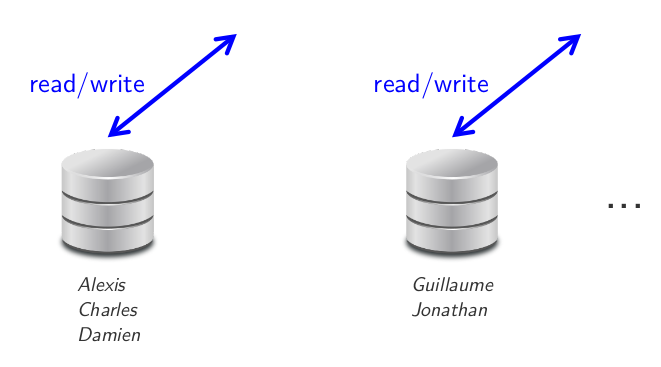
\includegraphics[scale=.3]{images/sharding}
\caption{Distribution des données: modèle sharding \cite{ref1}}
\end{figure}

\paragraph{Avantages:}
\begin{itemize}\setlength{\itemsep}{.2em}
\item[\textcolor{dkgreen}{\ding{52}}]fraction de la DB pour accélérer son traîtement et la rendre plus facile à gérer
\item[\textcolor{dkgreen}{\ding{52}}]avantages cluster (résistance aux pannes, \textit{scale out}, ...)
\end{itemize}

\paragraph{Inconvénients:}
\begin{itemize}\setlength{\itemsep}{.2em}
\item[\textcolor{dkred}{\ding{56}}]définir bonne répartition des données -> risque de surcharge d'un serveur
\item[\textcolor{dkred}{\ding{56}}]pas de résilience (ni en lecture, ni en écriture) -> si un serveur tombe, une partie de la DB n'est plus du tout accessible
\end{itemize}

}


%--- 25 -------------------------------%
\item\vf{Le sharding permet de récupérer les données en cas de corruption grâce à un stockage redondant
de ces dernières sur plusieurs serveurs pouvant être physiquement à des endroits différents.}
{\faux}
{En sharding les données ne sont pas répliquées contrairement aux modèles de réplications \textit{master/slave} ou \textit{peer-to-peer}.}


%--- 26 -------------------------------%
\item\vf{Réplication de données et sharding sont incompatibles.}
{\faux}
{Il est possible de combiner les techniques de \textit{sharding} et \textit{replication} ce qui offre les avantages de résilience (R, W ou les deux) et de répartition de la DB.
\paragraph{}
On peut combiner le sharding avec:
\begin{itemize}
\item[$\cdot$]le \textit{master/slave}: plusieurs maîtres (responsable chacun d'une partie de la DB) ou rôle mixtes (esclave pour certaines données et maîtres pour d'autres)
\item[$\cdot$]le \textit{peer-to-peer}: fraction de la DB (sharding) et réplication sur N noeuds
\end{itemize}
}


%--- 27 -------------------------------%
\item\vf{La réplication master-slave offre la propriété de résilience à la lecture.}
{\vrai}
{Dans le modèle de réplication master/slave, on distingue deux types de noeuds
\begin{enumerate}
\item le \textbf{master}: responsable des données et de leur mise à jour, il est accessible en R/W
\item les \textbf{slaves}: répliques complètes (!!) du maître, accessibles seulement en lecture
\end{enumerate}

\paragraph{}
Les requêtes des clients sont redirigées suivant que ce soit pour de la lecture ou de l'écriture. Comme le master est le seul accessible en lecture, il doit communiquer ses modifications aux esclaves pour les mettre à jour.

\paragraph{}
Ce modèle possède la propriété de \textit{read resilience}, càd que si le maître crash, le système sera toujours accessible en lecture via les esclaves. De plus, il est possible d'élir (manuellement ou automatiquement) un esclave comme nouveau maître si celui-ci tombe.

\begin{figure}[!h]
\center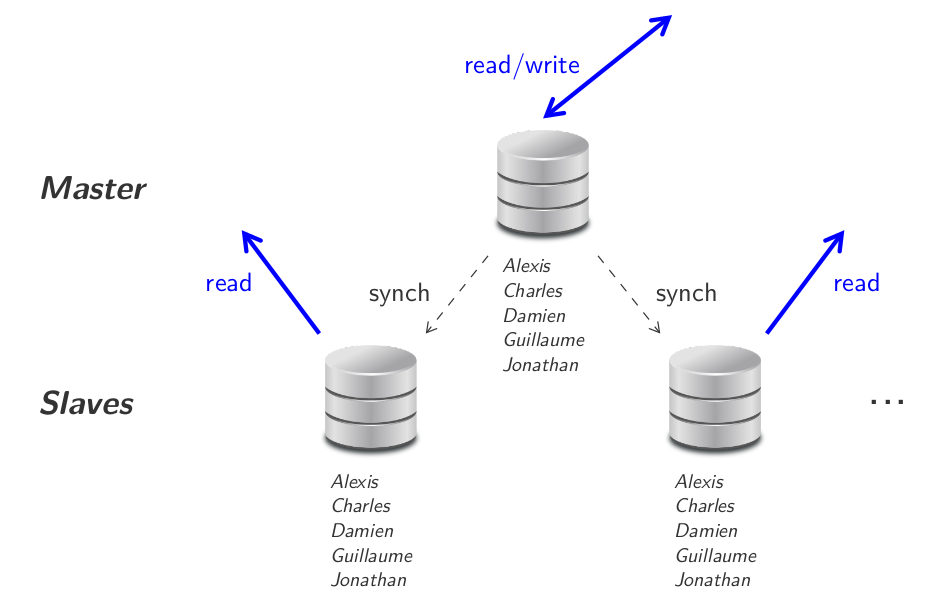
\includegraphics[scale=.3]{images/replication-masterslave}
\caption{Distribution des données: modèle de réplication master/slave \cite{ref1}}
\end{figure}

\paragraph{Avantages:}
\begin{itemize}\setlength{\itemsep}{.2em}
\item[\textcolor{dkgreen}{\ding{52}}]robustesse en cas de crash et \textit{read resilience}
\item[\textcolor{dkgreen}{\ding{52}}]fluidification du trafic pour les requêtes de lecture
\item[\textcolor{dkgreen}{\ding{52}}]avantages cluster (résistance aux pannes, \textit{scale out}, ...)
\end{itemize}

\paragraph{Inconvénients:}
\begin{itemize}\setlength{\itemsep}{.2em}
\item[\textcolor{dkred}{\ding{56}}]pas adapté lorsqu'il y a beaucoup d'écritures -> surcharge maître
\item[\textcolor{dkred}{\ding{56}}]nécessite plus d'espace de stockage puisque chaque noeud est une copie complète du maître
\item[\textcolor{dkred}{\ding{56}}]les valeurs lues par plusieurs utilisateurs peuvent être différentes par inconsistence -> la cohérence des données n'est pas garantie, puiqu'il faut que le maître ait synchronisé ses modifications avec les esclaves
\end{itemize}
}


%--- 28 -------------------------------%
\item\vf{En utilisant une réplication master-slave, les données deviennent complètement inaccessibles une
fois que le master tombe.}
{\faux}
{Par la propriété de \textit{read resilience}, les données seront toujours accessibles en lecture si le maître crash (avec risque de perte d'information si l'esclave n'était pas à jour par rapport au maître). Elles ne seront disponibles en écriture \textbf{que si} un esclave est désigné pour remplacer le maître (-> pas \textit{write resilience})}


%--- 29 -------------------------------%
\item\vf{La consistence des données est plus compliquées à garantir avec une réplication master-slave
qu’avec une réplication peer-to-peer.}
{\vrai}
{Dans le modèle de réplication \textit{peer-to-peer}, les noeuds sont tous égaux, ils sont \textbf{accessibles en lecture et en écriture}. A chaque écriture sur un noeud, tous les autres doivent être mis à jour, ce qui peut créer des conflits d'écriture concurrente si une même donnée est modifiée à deux endroits différents en même temps.
\begin{figure}[!h]
\center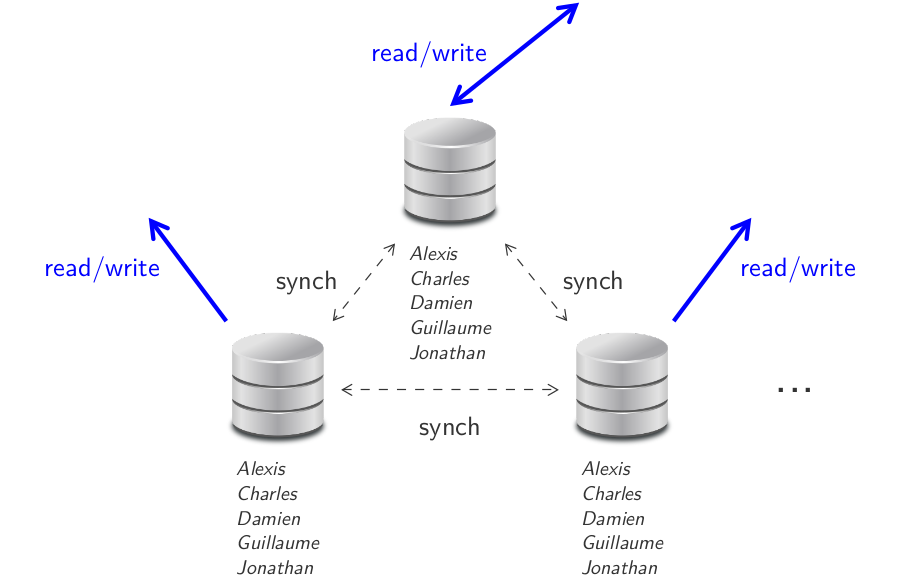
\includegraphics[scale=.3]{images/replication-peertopeer}
\caption{Distribution des données: modèle de réplication peer-to-peer \cite{ref1}}
\end{figure}

\paragraph{Avantages:}
\begin{itemize}\setlength{\itemsep}{.2em}
\item[\textcolor{dkgreen}{\ding{52}}]robustesse en cas de crash et \textit{complete resilience}
\item[\textcolor{dkgreen}{\ding{52}}]fluidification du trafic pour les requêtes de lecture ET d'écriture
\end{itemize}

\paragraph{Inconvénients:}
\begin{itemize}\setlength{\itemsep}{.2em}
\item[\textcolor{dkred}{\ding{56}}]pas adapté lorsqu'il y a beaucoup d'écritures -> lourdeur synchronisations
\item[\textcolor{dkred}{\ding{56}}]nécessite plus d'espace de stockage puisque chaque noeud contient toute la DB
\item[\textcolor{dkred}{\ding{56}}]risques de conflits d'écritures concurrentes
\item[\textcolor{dkred}{\ding{56}}]peu évoluable -> l'ajout d'un nouveau noeud impose de le connecter à TOUS les autres noeuds existants
\end{itemize}
}


%--- 30 -------------------------------%
\item\vf{La consistence des données est plus compliquées à garantir avec une réplication peer-to-peer
qu’avec une réplication master-slave.}
{\faux}
{En master/slave, les modifications peuvent \textbf{seulement} être effectuées via le maître. Il y a donc des risques d'inconsistence des données le temps que les esclaves soient mis à jour MAIS les modifications seront partout les mêmes.
\paragraph{}
En peer-to-peer, des modifications peuvent être faites \textbf{sur n'importe quel noeud} qui communique ensuite à tous les autres ses modifications. Des écritures concurrentes sur différents noeuds peuvent donc engendrer des problèmes d'inconsistence de données qui sont plus difficile à vérifier. (Rem: une solution serait de synchroniser tous les noeuds sur une même date/heure et d'utiliser un serveur dédié pour stocker les informations de mise à jour des données. Ainsi, on peut facilement déterminer la plus récente)
}

%--- 31 -------------------------------%
\item\vf{En utilisant une réplication master-slave, une lecture sur le master assurera toujours d’obtenir
les données les plus récentes}
{}
{}


%--- 32 -------------------------------%
\item\vf{Les buckets de Riak permettent de segmenter les données en plusieurs collections d’agrégats.}
{}
{}


%--- 33 -------------------------------%
\item\vf{On ne peut pas stocker des arbres binaires comme valeurs avec Redis.}
{}
{}


%--- 34 -------------------------------%
\item\vf{Redis garantit la persistance de données.}
{}
{}


%--- 35 -------------------------------%
\item\vf{Les bases de données orientée colonnes optimisent le stockage disque pour des tables qui
contiennent de nombreuses lignes.}
{}
{}


%--- 36 -------------------------------%
\item\vf{Une base de données orientée colonnes est très adaptée lorsqu’on a plus d’opérations d’écriture
que de lecture.}
{}
{}


%--- 37 -------------------------------%
\item\vf{Une base de données orientée colonnes est très adaptée lorsqu’on a plus d’opérations de lecture
que d’écriture.}
{}
{}


%--- 38 -------------------------------%
\item\vf{Une base de données orientée colonnes est un map à deux niveaux.}
{}
{}


%--- 39 -------------------------------%
\item\vf{Dans une base de données orientée colonnes, les familles de colonnes sont de préférence définies
une fois pour toute lors de la création de la table.}
{}
{}


%--- 40 -------------------------------%
\item\vf{L’avantage de l’utilisation de colonnes plutôt que de lignes est d’offrir une vitesse d’écriture plus grande de nouveaux enregistrements.}
{}
{}

\end{enumerate}



%------------------------------------------------------------------------
\chapter{Questions ouvertes}
%------------------------------------------------------------------------
Petite question rapide à répondre en une ou deux minutes maximum, sans devoir donner de détails,
juste pour s’assurer que vous avez compris le concept de la question.
\paragraph{}
\begin{enumerate}\setlength\itemsep{1em}
%--- 1 ----------------------------------------------------------
\item\qouv{Définissez ce qu’est un design pattern, comment le caractériser et à quoi il sert.}
{Un design pattern est un \textbf{modèle de conception} général qui répond à une problématique récurrente en développement. Il s'agit d'une desciption de solution dont l'implémentation doit être adpatée aux cas particulier.
\paragraph{}
Les patterns sont donc utilisés pour simplifier la vie des programmeurs, ils représentent un gain de temps (ne pas réinventer la roue) et une fiabilité puisqu'ils s'agit de modèles testés et approuvés avec le temps.

\paragraph{}
Un pattern est définit par:
\begin{itemize}
\item[$\cdot$]un \textbf{nom}
\item[$\cdot$]une \textbf{description du problème} auquel il s'applique
\item[$\cdot$]la \textbf{solution}: générique!! Son implémentation est à adapter au cas par cas
\item[$\cdot$]les \textbf{conséquences} de son utilisation: peut avoir des répercutions sur le reste du code, forcer des choix d'implémentation allieurs,...
\end{itemize}

\paragraph{}
Il existe 23 patterns \textit{classiques}, définis par le GoF, regroupés selon trois catégories:
\begin{enumerate}
\item \textbf{construction}: concerne l'instanciation des classes
\item \textbf{structuraux}: concerne l'organisation des classes entre elles
\item \textbf{comportementaux}: concerne la communication entre les objets
\end{enumerate}
}

%--- 2 ----------------------------------------------------------
\item\qouv{Que sont les concurrency patterns ? Donnez quelques exemples.}
{Ce sont des patterns utilisés pour de la \textbf{programmation concurrente}.
Ils apportent entre autre des modèles pour: la synchronisation, la communication, le stockage de données, les caches,...\paragraph{EXEMPLES [...]}
}

%--- 3 ----------------------------------------------------------
\item\qouv{Décrire ce qu’est le test driven development (TDD).}
{Le cycle TDD définit une méthode de développement qui consiste à être \textbf{guidé par l'écriture de tests} et intégrer des phases de refactoring.
\paragraph{}
La figure ci-dessous définit les trois grandes étapes de chaque tour de cycle. La deuxième étape consiste à écrire un code permettant de passer le(s) test(s) -> on ne parle encore d'optimisation. C'est seulement à l'étape 3, lorsque le code est fonctionnel, que l'on peut penser à des améliorations pour éliminer les \textit{bad smells}.
\begin{figure}[h!]
\center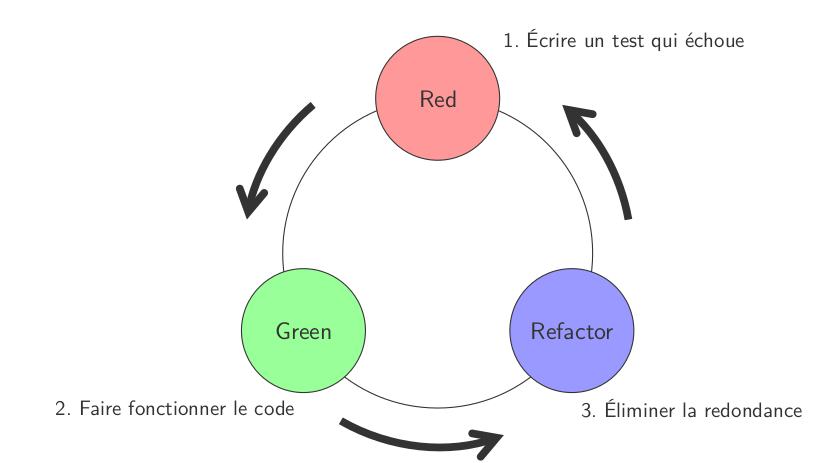
\includegraphics[scale=.4]{images/cycle-tdd}
\caption{Le cycle TDD selon Kent Beck}
\end{figure}

}

%--- 4 ----------------------------------------------------------
\item\qouv{Définissez ce qu’est un bad smell et donnez un exemple.}
{Un \textit{bad smell} est une \textbf{faiblesse de codage} dans un programme, il ne s'agit pas d'un bug!!!
\paragraph{}Exemples de bad smells:
\begin{itemize}\setlength{\itemsep}{.3em}
\item[$\cdot$] \textbf{Large class (the blob)}: une classe (God class) monopolise tout le traitement et les autres stockent uniquement des données -> va à l'encontre du principe de POO "une classe = une responsabilité". La \textit{God Class} utilise des détails d'implémentation des autres classes -> va à l'encontre de l'encapsulation.
\item[$\cdot$]\textbf{code dupliqué}: du code identique ou très similaire à différents endroits dans le programme -> difficile à maintenir. Il faut isoler les parties communes dans des métodes.
\item[$\cdot$]\textbf{Long method}: méthode dont le coprs possède beaucoup d'instructions -> limite la réutilisabilité et difficile à comprendre. Une méthode ne devrait avoir qu'une seule fonctionnalité.
\item[$\cdot$]...
\end{itemize}
}

%--- 5 ----------------------------------------------------------
\item\qouv{Définissez ce qu’est le refactoring et à quel moment il peut être utilisé dans le processus de
développement.}
{Le refactoring consiste à transformer du code tout en \textbf{préservant son comportement}, il s'agit donc d'\textbf{améliorer la qualité} d'un code déjà fonctionnel.
\paragraph{}
Cette technique s'inscrit dans la logique d'\textit{optimisation du code}, dont un principe fondamental est le suivant: \textit{"l'optimisation ne doit intervenir qu'une fois que le programme fonctionne et répond aux spécifications fonctionnelles."}
\paragraph{}
Dans le cas d'un cycle TDD (Test-Driven Development, voir Q3), le réfactoring du code a donc lieu après que celui-ci ait passé une batterie de tests. L'idée est de se servir de ces mêmes tests pour s'assurer que les modifications n'aient pas altéré le bon fonctionnement du code.

\paragraph{EXEMPLES [...]}

\paragraph{Remarque: }
l'étape de refactoring n'ajoute pas de fonctionnalité et ne corrige pas de bug !! On re-travaille un code dans le but d'améliorer sa lisibilité et sa maintenance mais son comportement externe reste identique.

}

%--- 6 ----------------------------------------------------------
\item\qouv{Définissez la notion de paradigme de programmation, ainsi que la programmation impérative et
déclarative.}
{}

%--- 7 ----------------------------------------------------------
\item\qouv{Définissez la notion de système distribué en reprenant rapidement les cinq buts.}
{}

%--- 8 ----------------------------------------------------------
\item\qouv{Définissez la notion de middleware. Dans quel type d’architecture les retrouve-t-on ?}
{}

%--- 9 ----------------------------------------------------------
\item\qouv{Donnez la différence entre un client léger et lourd, dans une architecture client-serveur.}
{}

%--- 10 ----------------------------------------------------------
\item\qouv{Qu’est-ce-que CORBA et quel type d’architecture supporte-t-il ?}
{}
%--- 11 ----------------------------------------------------------
\item\qouv{Quelles sont les différentes étapes de l’appel d’un service web ?}
{
L'architecture orientée-services (SOA) est un modèle d'architecture dans lequel les composants fournissent des services à des consommateurs (autres services où utilisateurs). Un service consiste en une \textbf{fonction bien définie} (avec ses limitations fonctionnelles et un rôle spécifique), \textbf{indépendante} et \textbf{mise à disposition} selon un "contrat" qui définit son utilisation.
\paragraph{}
Un service n'a pas d'état, il ne retient pas d'information sur les données qu'il traîte. Ainsi par exemple, un service de login permet d'authentifier un user mais il n'a pas conscience des users connectés, cela relève de la responsabilité de l'application.
\paragraph{}
Les données et les services, qui représentent la logique du système, sont \textbf{distribués}. Les services communiquent entre eux via des protocoles d'échanges de messages qui \textbf{suivent des standards}, ce qui assure le découplage et les rend facilement \textbf{réutilisables} pour former de nouveaux processus.
\paragraph{}
Les caractéristiques que doit satisfaire une telle architecture sont les suivantes:
\begin{enumerate}
\item avoir des \textcolor{ltred}{\textsc{frontières bien définies}}: 1 service = 1 fonctionnalité -> ensemble d'opérations définies
\item \textcolor{ltred}{\textsc{autonomie}} des services: les services doivent être indépendant, ce qui induit un faible couplage
\item les services partagent leur \textcolor{ltred}{\textsc{contrat}}: description du service -> ses fonctions et son utilisation
\item les services sont \textcolor{ltred}{\textsc{compatibles suivant des politiques}}: fonctionnalités du services changent selon contexte  (mise en page suivant navigateur web, gratuit/payant suivant utlisateur,...)
\end{enumerate}

\paragraph{}
Un "\textit{service web}" est un protocole qui permet à des applications, aux fonctionnalités diverses, d'échanger des données entre elles, il implémentate une architecture SOA . La figure \cite{appel-service-web} décrit la procédure d'appel d'un service web.
\paragraph{}
Différentes technologies sont utilisées par les services webs:
\begin{enumerate}
\item \textcolor{ltred}{\textsc{HTTP(s)}} (\textit{\textbf{H}yper\textbf{T}ext \textbf{T}rasnfert \textbf{P}rotocol \textbf{S}ecure}): communications
\item \textcolor{ltred}{\textsc{XML}} (\textit{e\textbf{X}tensible \textbf{M}arkup \textbf{L}anguage}) ou \textcolor{ltred}{\textsc{JSON}} (\textit{\textbf{J}ava\textbf{S}ript \textbf{O}bject \textbf{N}otation}): construction messages
\item \textcolor{ltred}{\textsc{WSDL}} (\textit{\textbf{W}eb \textbf{S}ervices \textbf{D}escription \textbf{L}anguage}): description précise des signatures (\textit{quoi}, \textit{où}, \textit{comment}) des services invoquables
\item \textcolor{ltred}{\textsc{UDDI}} (\textit{\textbf{U}niversal \textbf{D}escription, \textbf{D}iscovery, and \textbf{I}ntegration}): annuraire des services disponibles, protocole d'enregistrement des services
\item \textcolor{ltred}{\textsc{SOAP}} (\textit{\textbf{S}imple \textbf{O}bject \textbf{A}ccess \textbf{P}rotocol}): protocole d'invocation des messages
\end{enumerate}

\begin{figure}[h!]
\center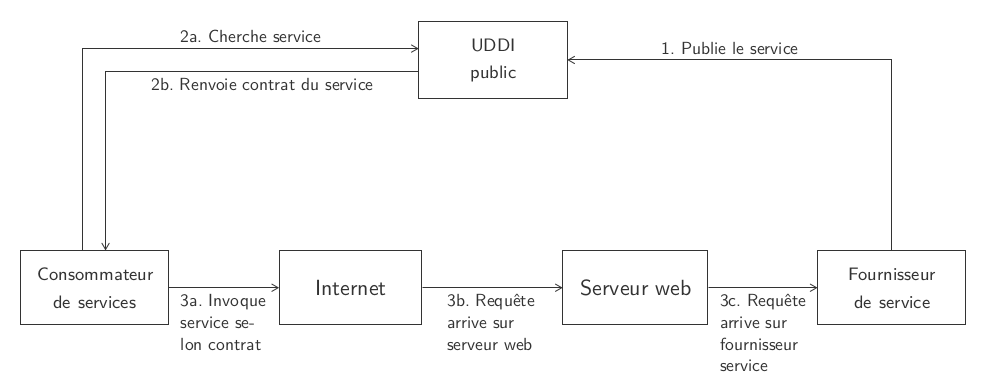
\includegraphics[scale=.4]{images/services-web}
\caption{Protocole d'appel d'un service web \cite{ref1}}
\label{appel-service-web}
\end{figure}

\paragraph{}Description des étapes:
\begin{enumerate}
\item \textcolor{ltred}{\textsc{publication du service}}: le fournisseur de service rapporte à l'annuaire sa présence. Autrement dit, il se fait connaître sur le réseau.
\item \textcolor{ltred}{\textsc{Recherche de service}} et \textcolor{ltred}{\textsc{envoie du contrat}}: Le consommateur interroge le répertoire de services pour prendre connaissance des services disponibles et connaître leurs contrats, c'est-à-dire la façon de les utiliser. Cette étape est nécessaire uniquement lors de la première utilisation d'un service (ou de temps en temps par après pour vérifier d'éventuelles mises à jour).
\item \textcolor{ltred}{\textsc{invocation du service}}: le consommateur fait appel au service selon les conditions définies par le contrat. La requête passe par le réseau Internet et arrive au serveur qui contient le code source pour exécuter le service.
\item \textcolor{ltred}{\textsc{réponse du service}}: le service effectue ses opérations et retourne une réponse au consommateur.
\end{enumerate}
}


%--- 12 ----------------------------------------------------------
\item\qouv{Expliquez brièvement les six contraintes d’une architecture REST ?}
{
REST (\textit{\textbf{RE}presentation \textbf{S}tate \textbf{T}ransfer}) est une architecture dédiée au développement de services web. Il s'agit d'une \textbf{collection de principes/contraintes/conventions} qui ne consitutent pas des standards (ce n'est pas une technologie en soi!) Autrement dit, leur utilisation n'est pas obligatoire pour l'implémentation d'un tel service.
\paragraph{}
L'architecture REST est définie par 6 principes:
\begin{enumerate}\setlength{\itemsep}{.3em}
\item\textcolor{ltred}{\textsc{uniform interface}}: interface uniforme entre le client et le serveur où les ressources sont identifiées par un \textbf{URI} (\textit{\textbf{U}niform \textbf{R}essource \textbf{I}dentifier}). Les requêtes reposent sur l'utilisation du \textbf{protocole HTTP} avec une hiérarchie des ressources et des \textit{query string} uniquement en tant que filtres (\textit{ex: \textcolor{dkyellow}{GET} http://www.example.com/\textcolor{purple}{customers/1234/orders}\textcolor{dkgreen}{?offset=0\& limit=25}}).

\item\textcolor{ltred}{\textsc{state less}}: le service n'a pas d'état, il ne conserve pas l'état des ressources, il n'existe donc pas de session entre le serveur et le client. C'est la \textbf{requête} (donc responsabilité côté client/application) qui \textbf{contient toute l'information} nécessaire à son traitement.\paragraph{}Ce principe permet de facilement déployer le service sur différents serveurs, le client pouvant alors être indifféremment redirigé vers l'un d'entre eux. En revanche, cela implique une mise en place correcte de la sémantique de l'application, puisque le serveur perd une partie du contrôle.

\item\textcolor{ltred}{\textsc{cacheable}}: possibilité de mettre une réponse en cache (côté serveur ou client) pour \textbf{augmenter les performances}. Ces informations en mémoire évitent de formuler des requêtes inutilement ou de traiter des requêtes identiques, mais avec un risque que celles-ci soient obsolètes (à contrôler).

\item\textcolor{ltred}{\textsc{client-serveur}}: \textbf{séparation précise des responsabilités} du serveur et du client, ce qui leur permet d'évoluer indépendamment.

\item\textcolor{ltred}{\textsc{layered system}}: définitions de \textbf{couches}, de telle sorte qu'une couche n'ait accès qu'à des composant d'une couche avec laquelle elle communique directement.

\item\textcolor{ltred}{\textsc{code on demand}}: le serveur envoie le code (JavaScript,...) au client de telle sorte qu'il puisse faire varier les fonctionnalités du service en fonction du client. \textbf{Variation dynamqiue du service} en fonction du contexte d'utilisation. 
\end{enumerate}
\paragraph{}
Lorsque les 6 contraintes sont implémentées, on parle alors d'architecture \textit{RESTful}.

\paragraph{}
Les avantages d'une telle architecture sont les suivants:
\begin{itemize}\setlength{\itemsep}{.2em}
\item[\textcolor{dkgreen}{\ding{52}}]répartition des requêtes et meilleure tolérance aux pannes, dus à l'absence d'état et donc la duplication du service
\item[\textcolor{dkgreen}{\ding{52}}]soulagement 
\end{itemize}
}


%--- 13 ----------------------------------------------------------
\item\qouv{Exposez brièvement les différences entre IaaS, PaaS et Saas.}
{}


%--- 14 ----------------------------------------------------------
\item\qouv{Exposez brièvement les différences entre IaaS, PaaS et Saas.}
{}


%--- 15 ----------------------------------------------------------
\item\qouv{Comment se calcule la complexité Fan-in Fan-out et quels sont ses avantages et inconvénients ?}
{La complexité "Fan-in Fan-out" est un \textit{métrique} qui se base sur le flux des données locales (in=params et out=valeurs retour).
\paragraph{}
Deux variantes existent pour calculer cette valeur de complexité:
\begin{enumerate}
\item \textbf{Henry et Kafura}: $HK = Length * (Fan_{in} * Fan_{out})^{2}$
\item \textbf{Shepperd}: $S = (Fan_{in} * Fan_{out})^{2}$
\end{enumerate}

\paragraph{UTILITE [...]}
}


%--- 16 ----------------------------------------------------------
\item\qouv{Définissez les notions de couplage afferent et efferent. Comment construit-on l’instabilité à partir
de ces métriques.}
{}

%--- 17 ----------------------------------------------------------
\item\qouv{Qu’est-ce-que la distance from main sequence et que permet-elle de mesurer ?}
{}

%--- 18 ----------------------------------------------------------
\item\qouv{Définissez brièvement les principes DRY et WET.}
{}

%--- 19 ----------------------------------------------------------
\item\qouv{Définissez le concept d’orthogonalité. En quoi améliore-t-il la qualité d’un logiciel ?}
{}

%--- 20 ----------------------------------------------------------
\item\qouv{Expliquez brièvement le principe du code traçant.}
{}
%--- 21 ----------------------------------------------------------
\item\qouv{Définissez brièvement la notion de microservice. }
{}

%--- 22 ----------------------------------------------------------
\item\qouv{L’architecte est un jardinier ou un planificateur de ville, expliquez.}
{}

%--- 23 ----------------------------------------------------------
\item\qouv{Quelles sont les différences entre principe et pratique.}
{}

%--- 24 ----------------------------------------------------------
\item\qouv{Qu’est-ce-qu’un contexte borné et quel est le lien avec microservice ?}
{}

\end{enumerate}


%------------------------------------------------------------------------
\chapter{Réflexion}
%------------------------------------------------------------------------
Pour les différentes questions ouvertes, ce qui est attendu est une discussion argumentée et appuyée
par des concepts vus au cours. N’hésitez pas à rappeler les définitions des concepts de base que vous
utiliserez dans votre argumentation. Il n’y a pas forcément de réponse unique aux questions de réflexion,
et ce qui sera évalué est l’exactitude de vos propos et l’utilisation adéquate d’arguments pertinents.
\paragraph{}
\begin{enumerate}\setlength\itemsep{1em}
%--- 1 -----------------------------------------------------------------------
\item\qouv{Il existe un lien fort entre l’architecture et la qualité d’un système logiciel. En particulier,
améliorer la qualité logicielle peut se faire en choisissant une architecture pertinente par rapport
au cahier des charges du système à développer. Expliquez en donnant des exemples concrets, et
argumentez.}
{}

%--- 2 -----------------------------------------------------------------------
\item\qouv{L’architecte logiciel est le garant de l’intégrité conceptuelle du système logiciel. De quoi
s’agit-il ? Quelles sont les différents éléments auquel il devra faire attention tout au long de la
durée de vie du logiciel ? Illustrez vos explications avec des exemples concrets, et argumentez.}
{}

%--- 3 -----------------------------------------------------------------------
\item\qouv{Décrivez brièvement les six principaux styles d’architecture suivant en donnant, pour chacun,
les avantages et inconvénients et un exemple concret utilisant ce style. Comparez ensuite ces
styles et déterminez une procédure qui permettrait à un architecte de se diriger vers le style le
plus adéquat étant donné un système logiciel à concevoir.
Centrée sur les données, flot de données, en couches, en niveaux, invocation implicite et MVC}
{}

%--- 4 -----------------------------------------------------------------------
\item\qouv{Le pattern d’implémentation argue qu’il faut viser l’excellence en programmation en suivant
les trois valeurs importantes que sont la communication, la simplicité et la flexibilité. En vous
appuyant sur des exemples de systèmes logiciel avec un choix d’architecture le plus adapté,
discutez à partir des avantages de l’architecture choisie de pourquoi elle permet de tendre vers
l’excellence.}
{}

%--- 5 -----------------------------------------------------------------------
\item\qouv{Un mauvais système logiciel peut se détériorer avec le temps avec pour conséquence qu’il
deviendra cher et difficile, voir impossible, à maintenir. L’une des causes majeures est que le
code a été sous-ingénierié. Qu’est-ce-que cela signifie-t-il et quelles sont les principales raisons
pouvant mener à un tel code ? Quelles bonnes pratiques, tant au niveau du code qu’au niveau de
l’architecture, peuvent aider à éviter un code sous-ingénieré ? Argumentez.}
{}

%--- 6 -----------------------------------------------------------------------
\item\qouv{Lorsqu’il s’agit de choisir un ou des langage(s) de programmation concret pour développer un
système logiciel, quelles sont les questions à se poser ? Comment peut-on organiser et structurer
la réflexion qui va guider vers le choix de langage ? Expliquez et argumentez.}
{}

%--- 7 -----------------------------------------------------------------------
\item\qouv{Dans les architectures orientée-interaction le système logiciel est découpé en trois partitions
principales : données, contrôle et vue. Comparez les trois grandes familles de modèles MV*
(MVC, MVVM et MVP) en identifiant comment les trois partitions sont organisées et identifiez
les avantages et inconvénients des différentes architectures existantes des trois familles.}
{}

%--- 8 -----------------------------------------------------------------------
\item\qouv{Les architectures de type broker et orientée-service possèdent une série de points communs,
notamment qu’elles permettent toutes deux de partager des services. Mais en quoi diffèrent-elles ?
Quels sont les avantages et inconvénients de ces deux types d’architecture ? Pour quel type
d’applications l’une ou l’autre sera-t-elle plus adaptée ? Argumentez.}
{}

%--- 9 -----------------------------------------------------------------------
\item\qouv{Les architectures prédominantes ont évolué avec les changements business partant de solutions
monolithiques vers des solutions actuellement orientées services. Expliquez comment cette
évolution s’est passée en reprenant les points forts et faibles de chacune des architectures de la
ligne du temps suivante et argumentez.}
{}

%--- 10 -----------------------------------------------------------------------
\item\qouv{Il y a trois principales architectures orientées données que sont le batch séquentiel, les pipes
et filtres et le contrôle de processus. Quels sont les points communs et différences entre ces trois
architectures, les avantages et inconvénients. Illustrez votre réponse à partir d’exemples concrets.
Quelles sont les questions que l’on pourrait se poser afin d’orienter son choix vers l’une des
trois architectures sachant qu’on a à réaliser un système logiciel qui doit traiter des données ?
Argumentez.}
{}
%--- 11 -----------------------------------------------------------------------
\item\qouv{Afin d’évaluer la complexité d’un système logiciel, on peut procéder à des mesures sur le
code de ce dernier. En particulier, on peut utiliser les métriques de Halstead, McCabe et Henry
ou Kafura/Shepperd pour mesurer différents types de complexité. Quels sont les aspects de complexité mesurés par ces métriques ? Comment sont elles calculées ? Discutez de la pertinence
des mesures ainsi réalisées, par rapport aux variables prises en compte et de l’utilité que l’on
peut faire de ces métriques.}
{}

%--- 12 -----------------------------------------------------------------------
\item\qouv{En quoi l’architecture en microservices permet-elle de suivre le principe de responsabilité
unique (SRP). Expliquez et argumentez en mentionnant les bénéfices d’une telle architecture.
En particulier, illustrez votre réponse en utilisant la notion d’architecture serverless et à l’aide
d’exemples concrets.}
{}

\end{enumerate}

\bibliographystyle{unsrt}
\bibliography{biblio}

\end{document}
